%%% use twocolumn and 10pt options with the asme2ej format
\documentclass[twocolumn,10pt]{asme2ej}
% \usepackage[italian]{babel}
\usepackage[utf8]{inputenc}
\usepackage{epsfig} %% for loading postscript figures
\usepackage{subfigure}
\usepackage{titling}
\usepackage{multicol}
\usepackage{booktabs}
\usepackage{siunitx}
\usepackage{amsmath}
\usepackage{tikz,mathtools}
\usepackage[hidelinks]{hyperref}
\usepackage{fancyhdr}
\pagestyle{fancy}
\renewcommand{\headrulewidth}{0pt}
\fancyhead{}
\fancyfoot{}
\fancyfoot[R]{\thepage}
\usepackage{caption}
\captionsetup[table]{name=Tab.}

\renewcommand{\tableautorefname}{Tab.}
\def\figureautorefname{Fig.} 
\def\equationautorefname{Eq.} 
\def\sectionautorefname{Sez.} 
\def\subsectionautorefname{Sez.} 
\def\subsubsectionautorefname{Sez.}


\pretitle{\begin{center}\linespread{1.2}\huge}
\posttitle{\par\end{center}\vspace{0.5em}}

\abovedisplayshortskip=0pt
\belowdisplayshortskip=0pt
\abovedisplayskip=-5pt
\belowdisplayskip=5pt

\newcommand{\tnhl}{\tabularnewline\hline}
\newcommand{\tn}{\tabularnewline}
\newcolumntype{x}[1]{%
	>{\centering\hspace{0pt}}p{#1}}%


%% The class has several options
%  onecolumn/twocolumn - format for one or two columns per page
%  10pt/11pt/12pt - use 10, 11, or 12 point font
%  oneside/twoside - format for oneside/twosided printing
%  final/draft - format for final/draft copy
%  cleanfoot - take out copyright info in footer leave page number
%  cleanhead - take out the conference banner on the title page
%  titlepage/notitlepage - put in titlepage or leave out titlepage
%  
%% The default is oneside, onecolumn, 10pt, final

\date{}
\title{{\huge\bfseries Laboratorio di Fisica} - {\LARGE A.A. 2020/2021} \\ 
    {\LARGE Docenti: A. Garfagnini - M. Lunardon} \\ {\Huge\bfseries Fotodiodo}}


%%% first author
\author{Cerrone Vanessa
    \affiliation{
    1200361\\
    vanessa.cerrone@studenti.unipd.it
    }	
}

%%% second author
\author{Cigagna Simone
    \affiliation{
	1193992\\
    simone.cigagna@studenti.unipd.it
    }	
}

%%% third author
\author{Lai Nicolò
    \affiliation{
	1193976\\
    nicolo.lai@studenti.unipd.it
    }	
}


\begin{document}


\maketitle    


% %%%%%%%%%%%%%%%%%%%%%%%%%%%%%%%%%%%%%%%%%%%%%%%%%%%%%%%%%%%%%%%%%%%%%%
\section{Introduzione}\label{s:introduzione}

Si vuole analizzare lo spettro dei fotoni emessi dall'Americio-241 con un rivelatore al Silicio tipo PIN, dotato di
preamplificatore di carica. L’hardware, cioè i moduli di elettronica, sono stati pre-impostati in condizioni standard,
con shaping time pari a $3\mu\si{\second}$, in modo da ottimizzare il rapporto segnale rumore. Preliminarmente, tramite
il software di acquisizione, si registra uno spettro per identificare i picchi principali, a 60keV e 14-18keV. \\

Nella \autoref{s:attenuazione} si analizzerà il picco a 59.5keV in presenza di materiali di diverso spessore, al fine di
calcolare i relativi coefficienti di assorbimento. Nella  \autoref{s:distanza}, si effettueranno misure al variare della
distanza della sorgente, per verificare che i dati seguano l'andamento atteso. Un'analisi dettagliata dello spettro
verrà presentata nella sezione \autoref{s:multipicco}. 

% scriviamo 60 59 59.5 keV ???



% %%%%%%%%%%%%%%%%%%%%%%%%%%%%%%%%%%%%%%%%%%%%%%%%%%%%%%%%%%%%%%%%%%%%%%
\section{Spettro dell'Am-241}\label{s:spettro}

Prima di studiare in dettaglio gli effetti di diversi assorbitori posti tra la sorgente ed il detector ed il ruolo che
svolge la distanza di quest'ultimo dalla prima, ci si vuole concentrare in un'analisi dello spettro dell'Americio-241.
Sperimentalmente, il rivelatore viene posto alla minima distanza dalla sorgente e non viene inserito alcun assorbitore
tra i due. Il tempo di acquisizione viene impostato a $600\,\si{\second}$, rivelando così approssimativamente $2 \cdot
10^5$ eventi con un rate istantaneo di circa $340\,\si{\hertz}$. In questo modo, il picco a
$60\,\si{\kilo\electronvolt}$ presenta una precisione $\sqrt{\text{N}}/\text{N} \approx 1.5\%$.

\subsection{Calibrazione e Risoluzione Energetica}\label{s:calibrazione}

Inizialmente, si vuole calibrare l'asse orizzontale riconoscendo nello spettro in \autoref{i:spettro} il picco a
$60\,\si{\kilo\electronvolt}$. Nel grafico è presentato lo spettro di emissione con l'asse calibrato in energia: per
ottenere tale risultato è stato eseguito un fit gaussiano del picco, come mostrato nel riquadro all'interno del grafico.
Ovviamente, la calibrazione ottenuta sfruttando unicamente il picco a $60\,\si{\kilo\electronvolt}$ e assumendo
l'assenza di un possibile offset è approssimata, tuttavia risulta essere sufficiente per gli scopi dell'esperienza. 

\begin{figure}
    \centering
    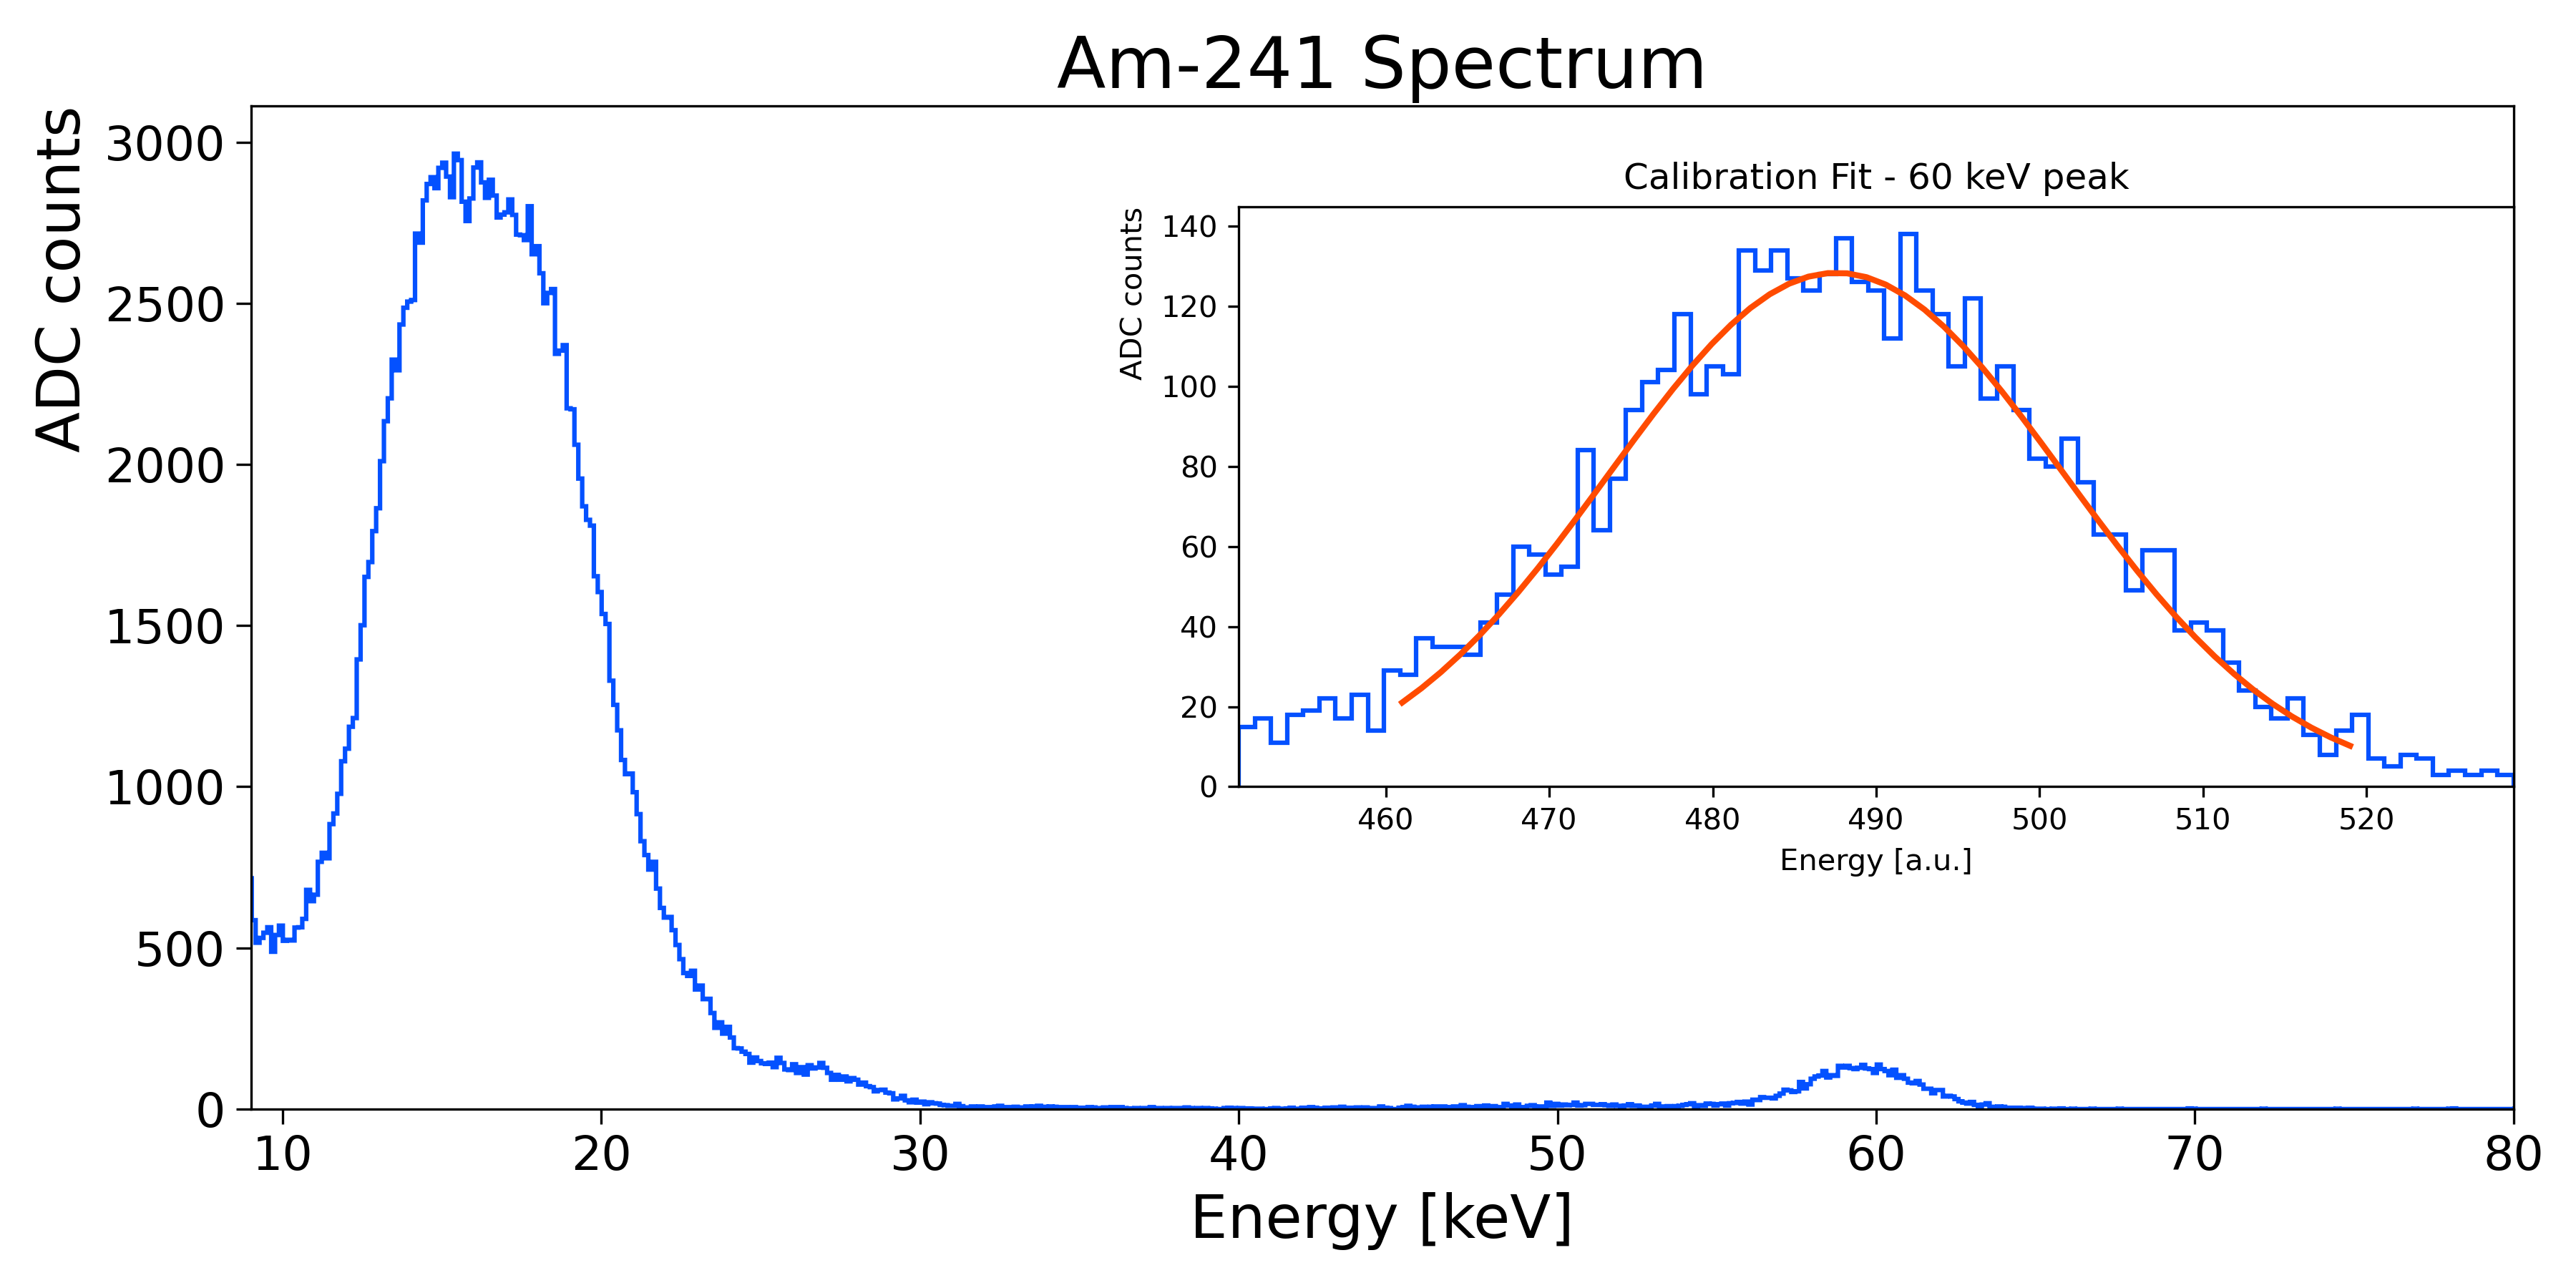
\includegraphics[width=\linewidth]{../Plots/am_spectrum_small.png}
    \caption{Spettro dell'Americio-241 con fit del picco a 60 keV per la calibrazione
               dell'asse orizzontale}
    \label{i:spettro}
    \vspace{-10pt}
\end{figure}

Dal fit del picco a $60\,\si{\kilo\electronvolt}$ è possibile infine estrapolare una stima approssimata della
risoluzione energetica R: 

\vspace{-15pt}
\begin{equation}
    \text{R} = \frac{\Delta\text{E}}{\text{E}}
    \underset{\mathllap{
      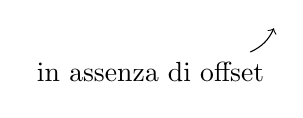
\begin{tikzpicture}
        \draw[->] (-0.3, 0) to[bend right=20] ++(0.3,2ex);
        \node[below left] at (0,0) {in assenza di offset};
      \end{tikzpicture}
    }}{\simeq}
    \frac{\text{FWHM}}{\text{mean}} = 6.75\%
\vspace{-5pt}
\end{equation}


\subsection{Fit Multi-Picco}\label{s:multipicco}

\begin{figure*}
    \centering
    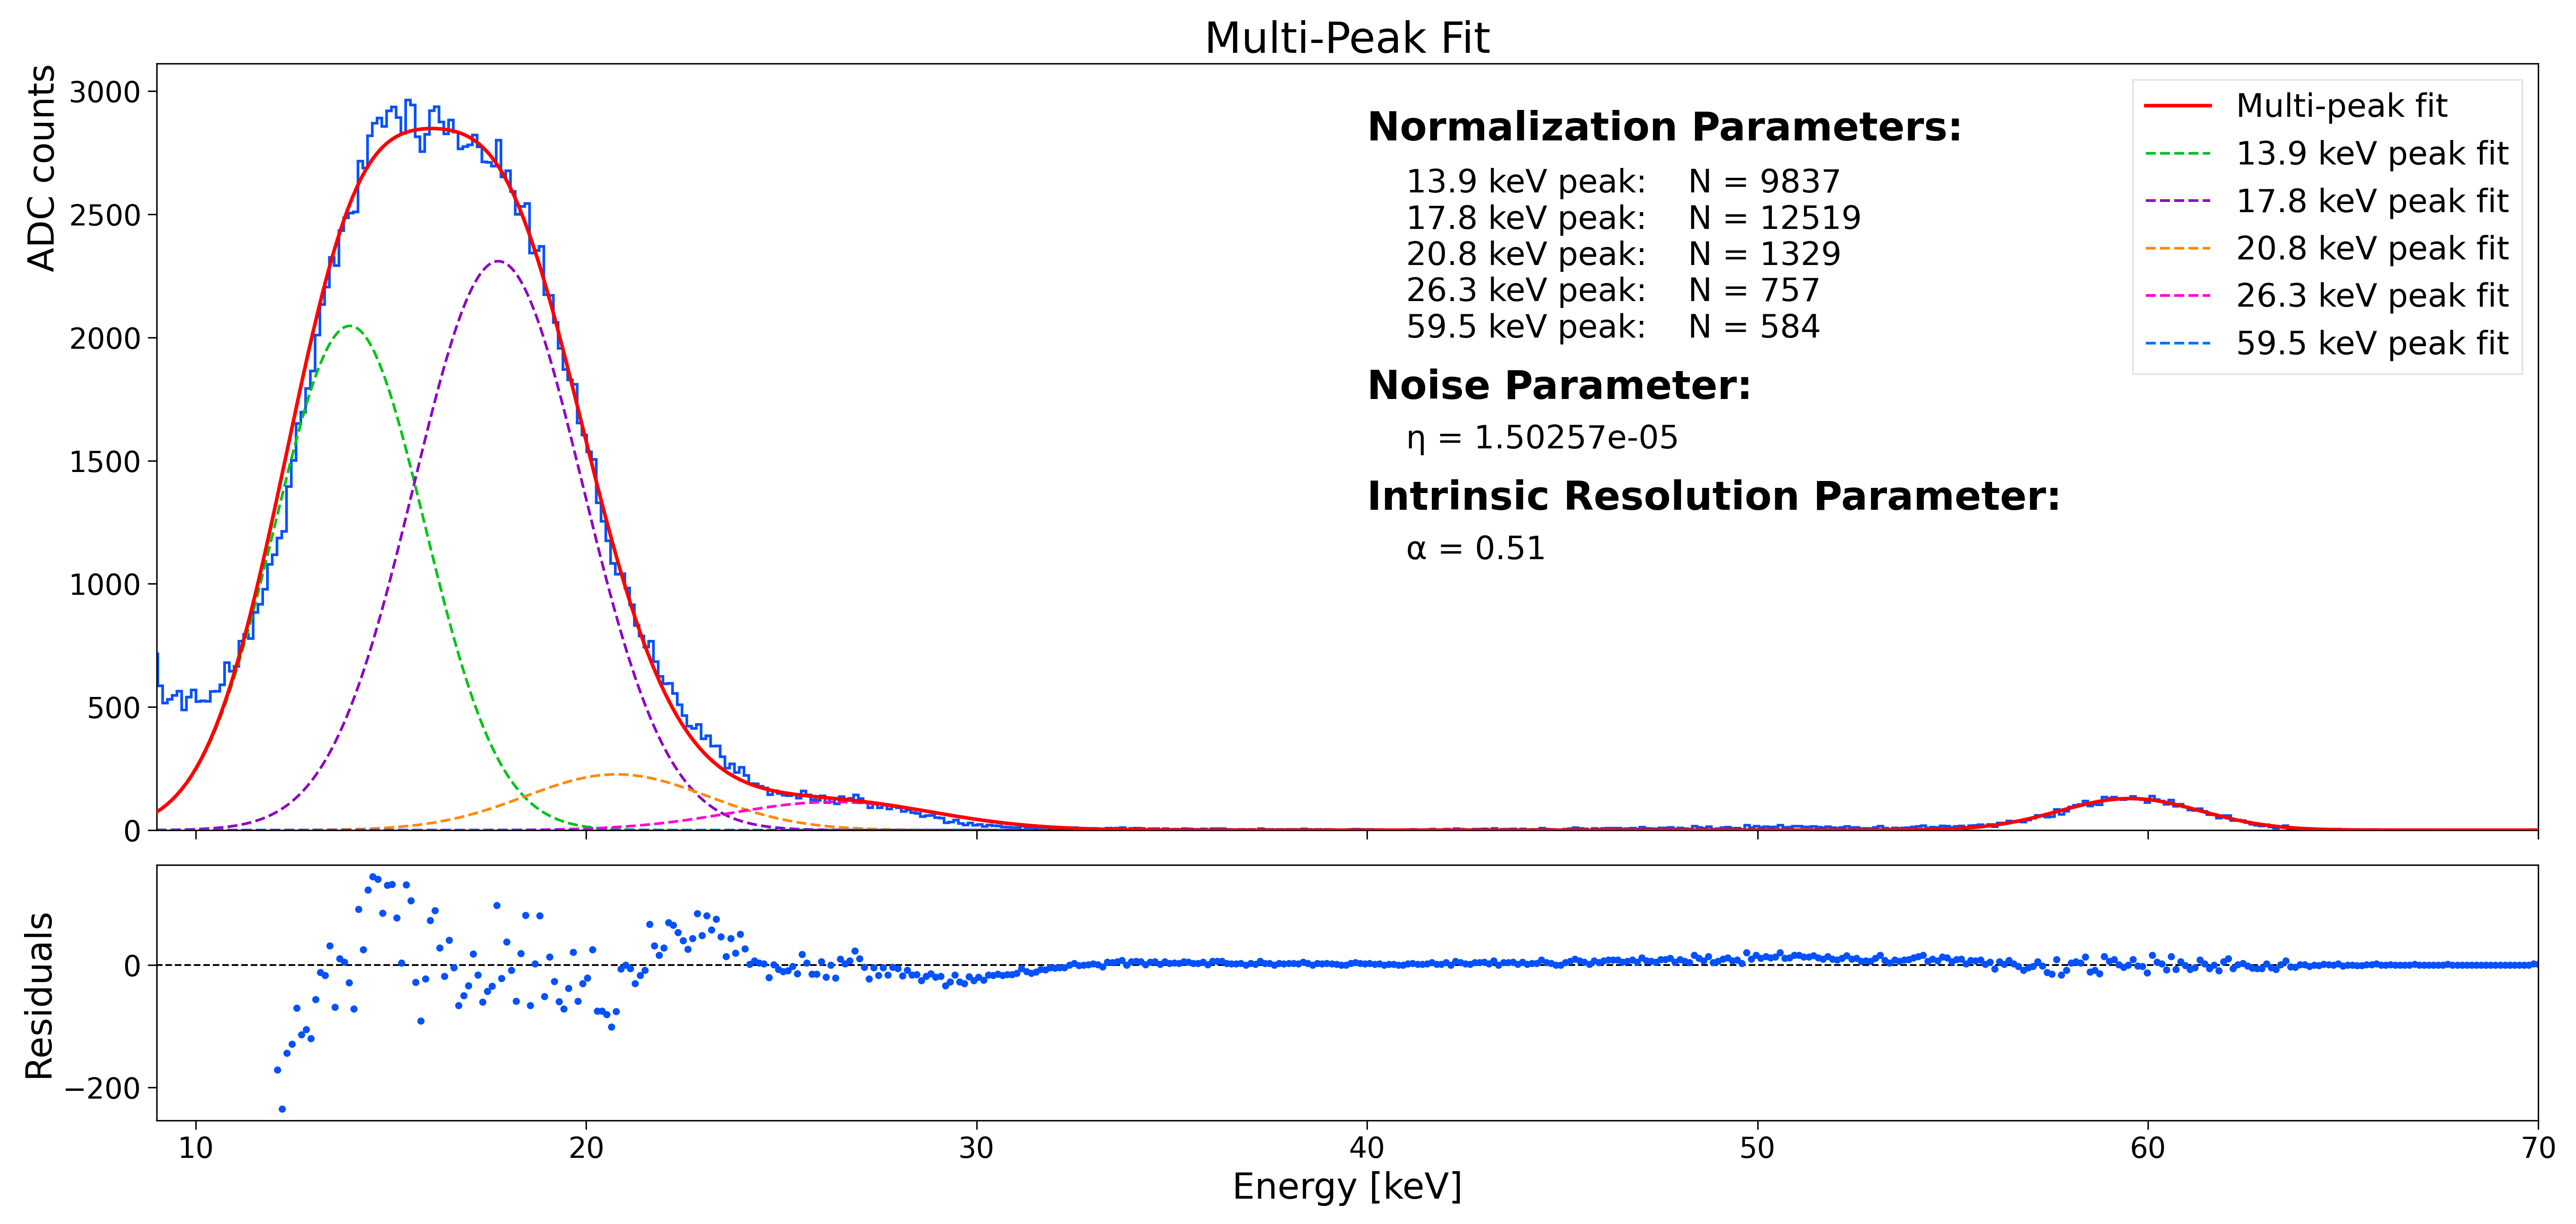
\includegraphics[width=\textwidth]{../Plots/multifit.png}
   \caption{Fit multi-picco dello spettro dell'Americio-241}
    \label{i:multifit}
    % \vspace{-10pt}
\end{figure*}

Ci si propone ora di costruire un fit complessivo di tutto lo spettro raffigurato in \autoref{i:spettro}. Ci si
concentra unicamente sulle emissioni di raggi X e gamma con un'intensità di almeno 2 fotoni ogni 100 disintegrazioni: in
\autoref{t:probabilities} sono riportati quindi i contributi considerati con le relative probabilità di emissione. Per
ciascuno di questi, si costruisce una funzione gaussiana con media fissata in quanto l'energia è nota
(\autoref{t:probabilities}) e l'asse orizzontale è stato preliminarmente calibrato. La larghezza della gaussiana
(sigma), invece, si compone di due contributi in somma quadratica: il primo è una componente fissa, di rumore, che verrà
denotata come $\eta$, mentre il secondo è la componente di risoluzione intrinseca $\alpha$ proporzionale alla radice
quadrata dell'energia del fotone preso in considerazione. \\
Il fit viene effettuato minimizzando un $\chi^2$ composto dalla somma quadratica dei singoli $\chi^2$ dati da ciascun
contributo gaussiano, ottendendo in questo modo quanto raffigurato in \autoref{i:multifit}. In particolare, sono stati
scelti come parametri liberi il contributo di rumore $\eta$ e di risoluzione intrinsceca $\alpha$, assieme ai fattori di
normalizzazione $\{\text{N}_i\}$ relativi ad ogni singolo picco considerato. Osservando quindi il grafico in
\autoref{i:multifit}, la curva in rosso rappresenta il fit complessivo dello spettro: questa segue in modo più che
soddisfacente il profilo delle emissioni dell'Am-241. Le curve tratteggiate, invece, corrispondono ai singoli contributi
gaussiani considerati per effettuare il fit: risulta quindi evidente che il potere risolvente dell'apparato non è
sufficiente per identificare tali contributi singolarmente. Dal grafico dei residui, relativi al fit complessivo, si può
notare una certa difficoltà nel seguire in modo fedele il profilo del primo picco, in quanto composto da numerosi
contributi. Il picco a $60\,\si{\kilo\electronvolt}$, invece, risulta in maggiore accordo con la funzione di regressione.



\begin{table}[t]
	\centering
	\begin{tabular}{x{3cm} x{3cm}} 

        \toprule[0.5px]
        \toprule[0.1px]

		\multicolumn{2}{c}{Probabilità di Emissione} \tn

		\midrule[0.1px]

		Energia [keV] & Prob. (\%) \tn

		\addlinespace

		13.9    & 11.60 (12)    \tn
        17.8    & 11.83 (12)    \tn
        20.8    & 2.94 (3)      \tn
        26.3    & 2.31 (8)      \tn
        59.5    & 35.92 (17)    \tn

		\bottomrule[0.5px]		
	\end{tabular}
	\caption{Energie dei fotoni considerati nel fit multi-picco e relative probabilità di emissione}
	\label{t:probabilities}
    \vspace{-10pt}
\end{table}	



% %%%%%%%%%%%%%%%%%%%%%%%%%%%%%%%%%%%%%%%%%%%%%%%%%%%%%%%%%%%%%%%%%%%%%%
\section{Coefficiente di assorbimento}\label{s:attenuazione} 

Ci si propone di effettuare delle misure in presenza di materiali di diverso spessore, nello specifico rame e argento,
con lo scopo di calcolarne il coefficiente di assorbimento $\mu$, che si ricava dalla relazione:

\vspace{-15pt}
\begin{equation}
   \text{I}(x) = \text{I}_0 \text{e}^{-\mu x}
    \vspace{-5pt}
    \label{e:mu}
\end{equation}

dove I è l'intensità della radiazione incidente e x lo spessore attraversato. In particolare, si vuole fornire una stima
del coefficiente di assorbimento massivo, definito come:

\vspace{-15pt}
\begin{equation}
   \mu_{\rho} = \frac{\mu}{\rho}
    \vspace{-5pt}
    \label{e:mu_mass}
\end{equation}

con $\rho$ densità del materiale, che è pari a 10.49$\si{\gram \cdot \centi\metre ^{-3}}$ per l'argento
e 8.96$\si{\gram \cdot \centi\metre ^{-3}}$ per il rame. 
\\ Si inseriscono gli assorbitori di spessore variabile e si acquisiscono gli spettri per
un intervallo di tempo sufficiente a garantire una precisione migliore del 3\% sul picco a 59.5keV.
La precisione in percentuale si ottiene ricavando il numero di eventi N, cioè l'area, al di sotto del
picco di interesse, come $\frac{\sqrt{\text{N}}}{\text{N}}$. 
% questa formula è da giustificare, viene da distribuzione di Poisson? 
Si calcola il rate degli eventi nel picco a 60 keV per tutte le misure effettuate come rapporto tra numero di 
eventi rilevati e tempo di acquisizione, che come prima è stato adattato in modo da avere precisioni di almeno il 3\%.
Considerando la relazione \autoref{e:mu} si effettua un fit del rate in funzione dello spessore del materiale, 
separatamente per rame e argento. Si sottolinea che il rapporto N/t rappresenta l'intensità della radiazione incidente
per unità di superficie: il rivelatore a disposizione ha un'area di 1$\si{\centi\metre}^2$, dunque il fit restituisce 
parametri dimensionalmente corretti. (?) \\


\begin{figure*}[t]
    \centering
    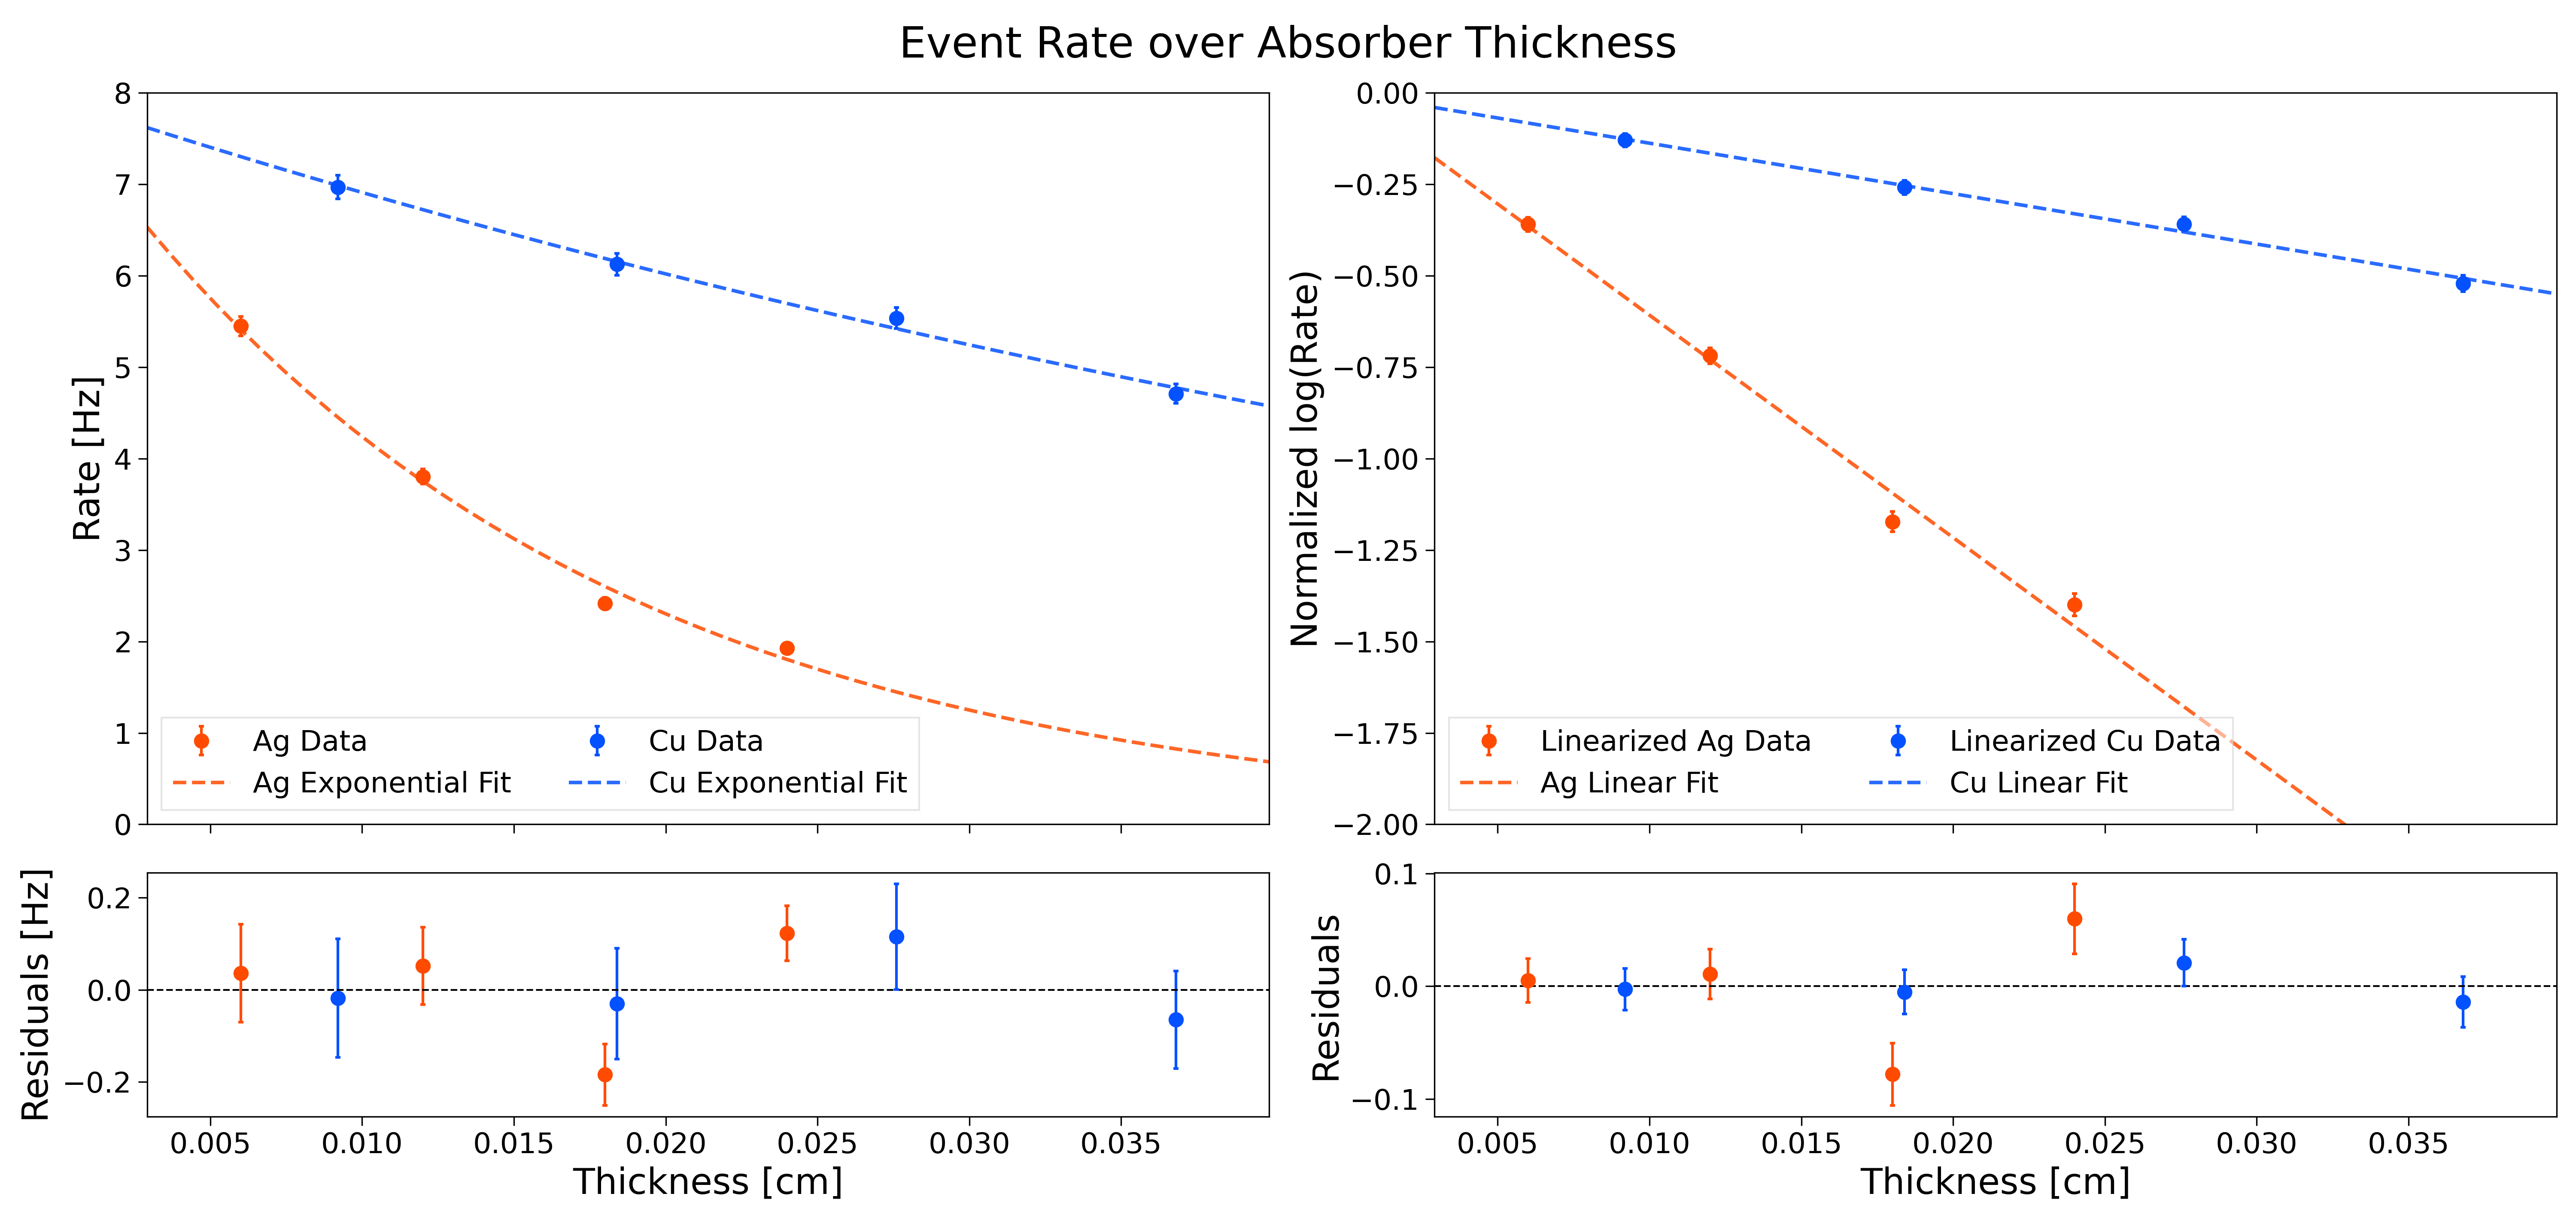
\includegraphics[width=\textwidth]{../Plots/attenuation_coeff.png}
   \caption{A sinistra fit esponenziale, a destra fit linearizzato per il calcolo dei coefficienti di assorbimento}
    \label{i:attenuation}
    % \vspace{-10pt}
\end{figure*}

Si riportano in \autoref{t:assorbimento} i dati utilizzati per l'interpolazione, con errore sulle ordinate calcolato per 
propagazione, trascurando le incertezze sui tempi di acquisizione. Infatti, alla luce del fatto che i valori dei tempi di
acquisizione mostrati sull'interfaccia del software si discostavano senibilmente da quelli impostati manualmente, si è 
assunto un errore massimo di 0.1\si{\second}, ed è stato preliminarmente verificato che tale contributo avesse un peso 
relativo trascurabile. SI Vuole inizialmente effettuare un fit esponenziale del tipo $y = \text{I}_0 \text{e}^{-\mu x }$. 
Successivamente, sfruttando il parametro $\text{I}_0 $ per normalizzare i dati, si vuole considerare il logaritmo delle 
intensità normalizzate ed effettuare una regressione lineare con la retta  di equazione y = m$x$  In questo modo, quindi, 
i dati si distribuiscono secondo $\log(\text{I}/\text{I}_0)=-\mu x$, con errore sul logaritmo ottenuto per propagazione. \\
Si riportano i parametri ottenuti in ... Si vuole ora quantificare la bontà dei fit: nel caso dell'argento si nota che 
il $\chi^2$ risulta significativamente maggiore rispetto ai gradi di libertà, sia nel fit esponenziale che in quello lineare
(compatibilità rispettivamente $Z=5$ e $Z=3.7$). Tale discrepanza può essere dovuta principalmente ad una leggera 
sottostima delle incertezze sul rate e al basso numero di dati. Tuttavia, i residui si distribuiscono sufficientemente bene
attorno allo zero, perciò la stima dei parametri è da considerarsi valida. Per il rame, invece, si trova un ottimo accordo tra
$\chi^2$ e numero di gradi di libertà (compatibilità rispettivamente $Z=0.3$ e $Z=0.6$): infatti i dati seguono chiaramente
l'andamento atteso e gli errori sulle ordinate coprono bene la dispersione. 
\indent In riferimento ai risultati in tab., si computano i coefficienti di assorbimento massivi, da confrontare con i valori 
teorici: $\mu_{\rho}^{\text{th}}$(Ag) = 5.7660 $\si{\centi\metre^2\gram^{-1}}$ e
 $\mu_{\rho}^{\text{th}}$(Cu) = 1.593 $\si{\centi\metre^2\gram^{-1}}$. Si ottengono:

 \vspace{-15pt}
\begin{align*}
    \mu_{\rho}(\text{Ag}) &= 5.3\pm 0.2 \si{\centi\metre^2\gram^{-1}} & \lambda &= 0.3 \\
    \mu_{\rho}(\text{Cu}) &= 1.5\pm 0.1 \si{\centi\metre^2\gram^{-1}} & \lambda &= 0.5 
    \vspace{-5pt}
\end{align*}



\begin{table}[t]
    \begin{center}
        \resizebox{\linewidth}{!}{%
        \begin{tabular}{c c | c c}
            \multicolumn{2}{c}{\textbf{Ag}} & \multicolumn{2}{c}{\textbf{Cu}} \\ 
            \hline
            \multicolumn{1}{c}{Spessore [$\si{\micro\metre}$]} & \multicolumn{1}{c|}{Rate [Hz]} & \multicolumn{1}{c}{Spessore [$\si{\micro\metre}$]} & \multicolumn{1}{c}{Rate [Hz]} \\
            60                           & $5.45  \pm 0.11 $                    & 92                           & $6.97 \pm 0.13$                    \\
            120                          & $3.80  \pm 0.08 $                    & 184                          & $6.12 \pm 0.12$                    \\
            180                          & $2.42  \pm  0.07$                    & 276                          & $5.54 \pm 0.11$                      \\
            240                          & $1.93  \pm  0.06$                    & 368                          & $4.71 \pm 0.11$                      \\  
            \hline
        \end{tabular}%
            }
    \end{center}
    \caption{Dati fit esponenziale per il calcolo del coefficiente di assorbimento}
    \label{t:assorbimento}
\end{table}




% %%%%%%%%%%%%%%%%%%%%%%%%%%%%%%%%%%%%%%%%%%%%%%%%%%%%%%%%%%%%%%%%%%%%%%
\section{Legge dell'Inverso del Quadrato della Distanza}\label{s:distanza}

Ci si propone ora di verificare la cosiddetta "legge dell'inverso del quadrato della distanza". In particolare, si vuole
controllare che il rate dei raggi X (ovvero il primo picco a sinistra in \autoref{i:spettro}) segua un andamento
proporzionale all'inverso della distanza al quadrato tra sorgente e detector. In assenza di assorbitori tra i due,
quindi, vengono acquisiti una serie di spettri facendo variare la posizione del rivelatore. Dagli spettri acquisiti
viene calcolato il rate degli X: tali valori, assieme alla posizione del detector, sono riportati in
\autoref{t:distance}. Questi vengono quindi raffigurati in \autoref{i:distance}: si vuole far notare in particolar modo
la presenza di un parametro $x_0$ di zero. Infatti, tramite il software per la movimentazione del detector è possibile
unicamente impostarne la posizione lungo una rotaia: l'effettiva distanza con la sorgente è invece ignota a priori in
quanto la posizione della sorgente non corrisponde allo zero del sistema di riferimento utilizzato dal software per
posizionare il detector sulla guida. \\
Per la verifica della legge dell'inverso del quadrato della distanza si vuole quantificare la bontà del fit: il $\chi^2$
risulta sensibilmente maggiore rispetto ai gradi di libertà (compatibilità $Z=3$). Tuttavia, siccome nel caso in
questione non sono stati considerati numerosi effetti ulteriori e, possibilmente anche a causa dello scarso potere
risolvente dell'apparato, l'incertezza sul rate di rivelazione può essere stata (leggermente) sottostimata. In questo
caso, dunqe, una compatibilità $Z=3$ con i gradi di libertà non è da considerarsi pessima: osservando il grafico dei
residui, infatti, si osserva un soddisfacente andamento attorno allo zero. Si può quindi concludere che le misure
acquisite al variare della distanza tra sorgente e detector seguono piuttosto fedelmente un andamento proporzionale
all'inverso della distanza al quadrato. 

\begin{figure}
    \centering
    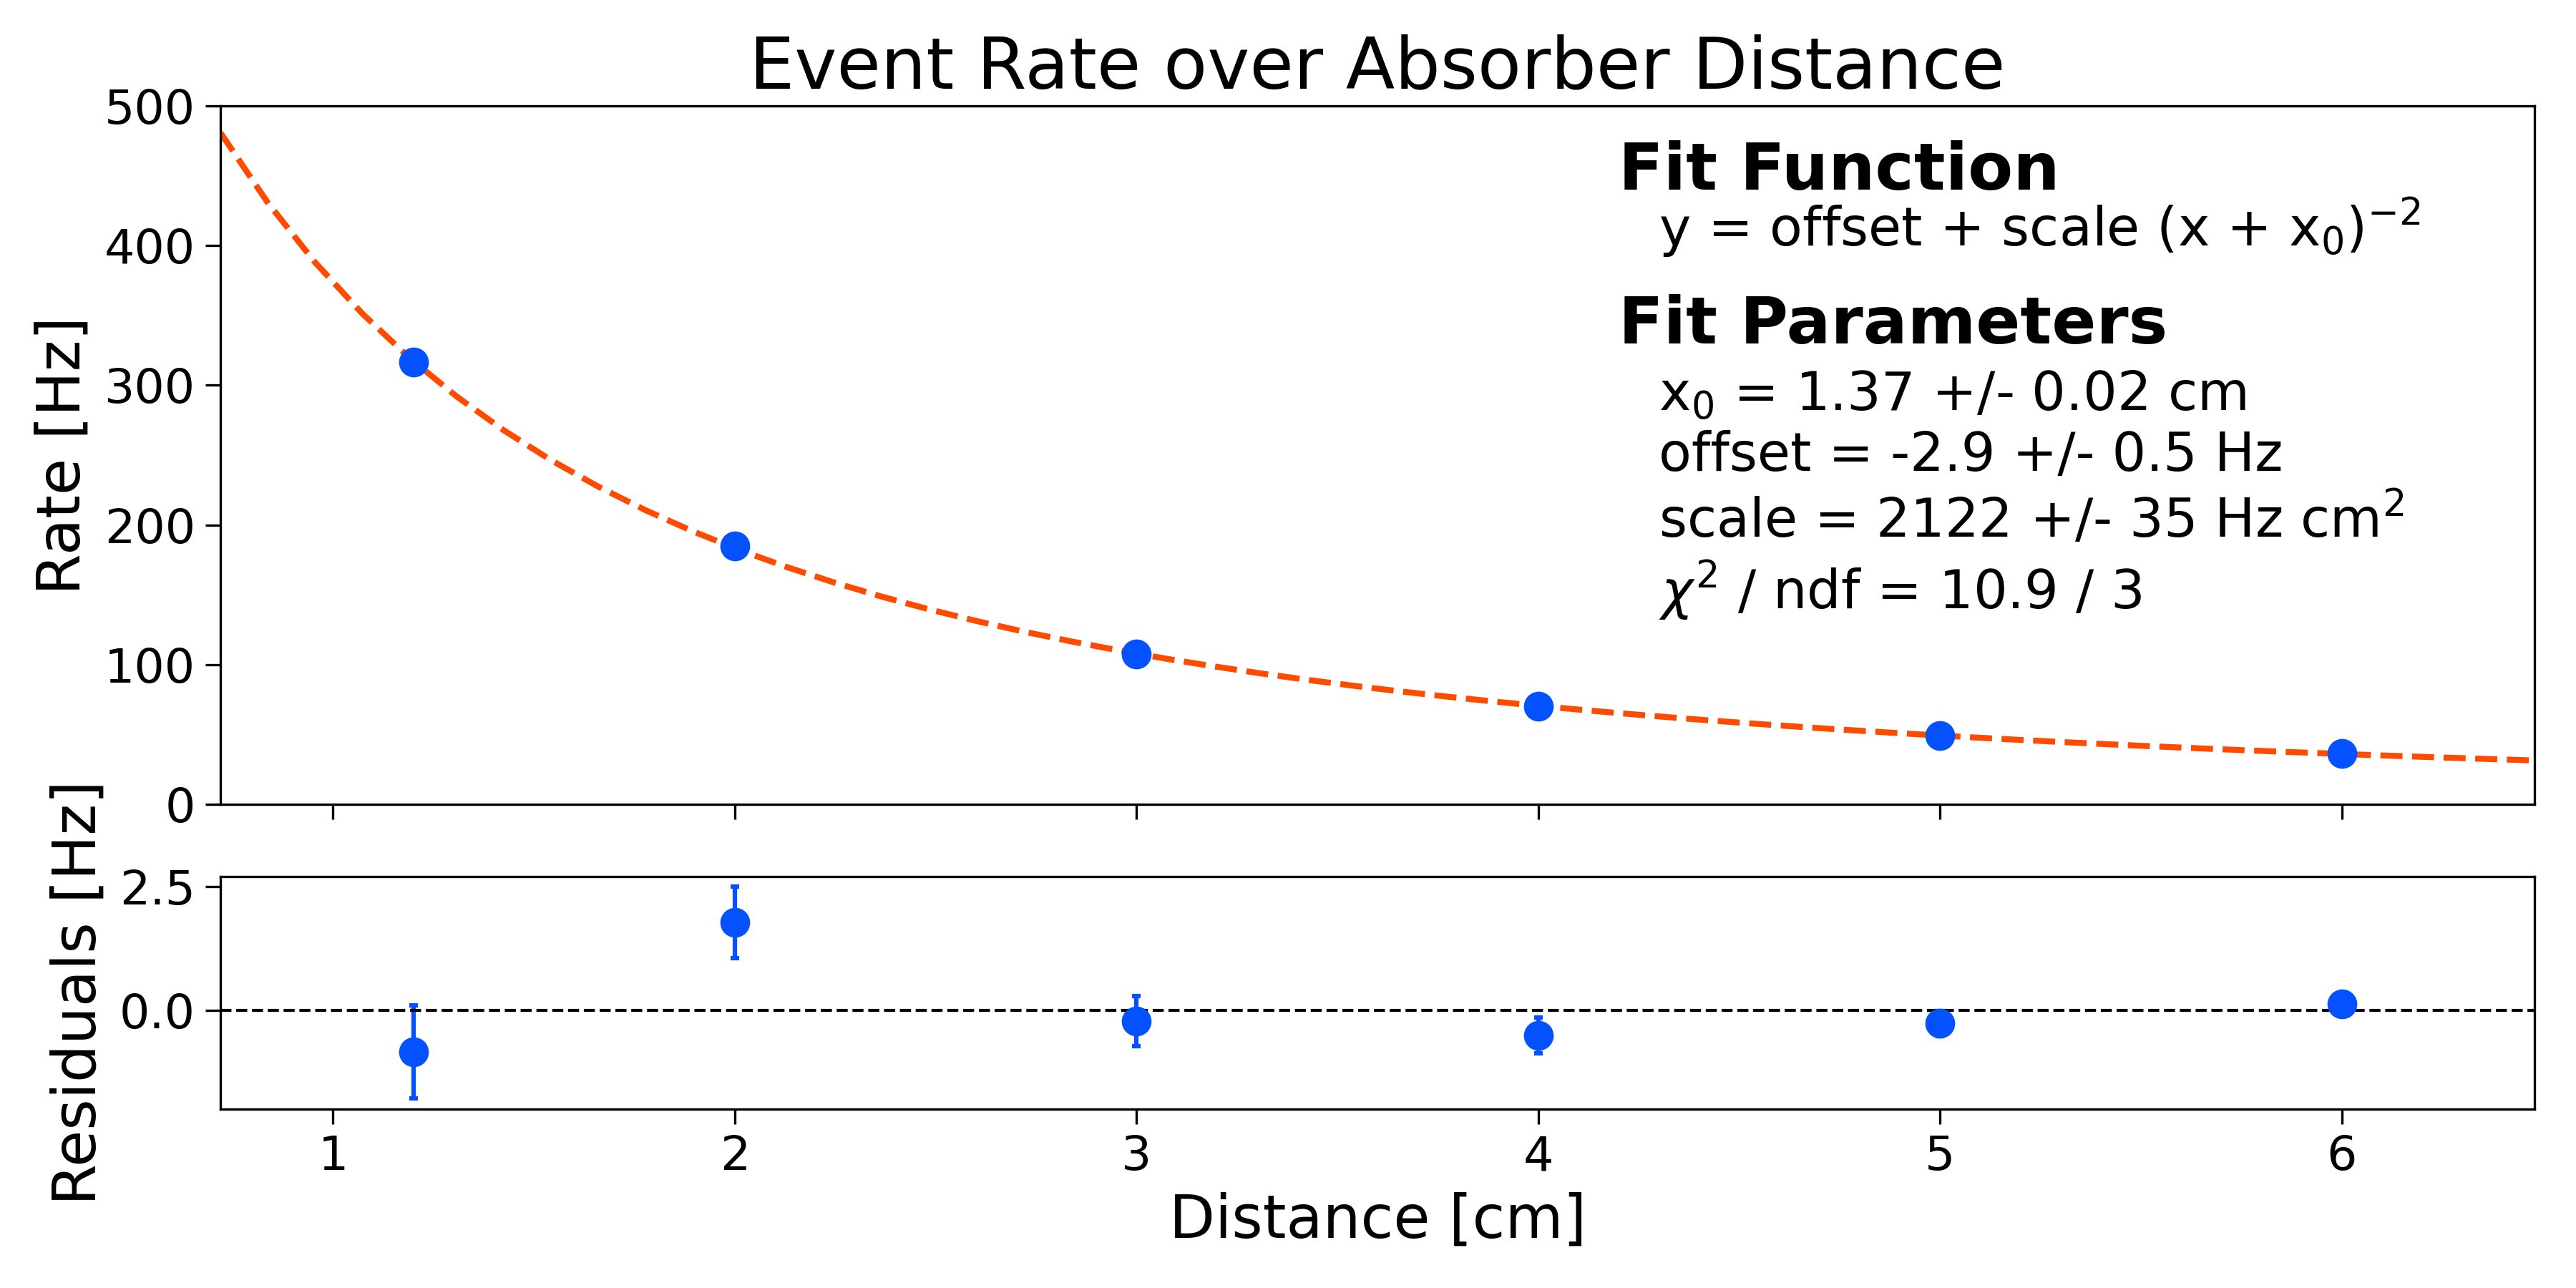
\includegraphics[width=\linewidth]{../Plots/distance_small.png}
    \caption{Rate di rivelazione dei raggi X in funzione della distanza tra sorgente e detector}
    \label{i:distance}
    \vspace{-10pt}
\end{figure}


\begin{table}[t]
	\centering
	\begin{tabular}{x{3cm} x{3cm}} 

        \toprule[0.5px]
        \toprule[0.1px]

		\multicolumn{2}{c}{Rate in funzione della posizione} \tn

		\midrule[0.1px]

		Posizione [cm] & Rate [Hz] \tn

		\addlinespace

        $1.2$	&   $316.4	\pm 0.9$ \tn
        $2.0$	&   $185.2	\pm 0.7$ \tn
        $3.0$	&   $107.8	\pm 0.5$ \tn
        $4.0$	&   $70.1	\pm 0.4$ \tn
        $5.0$	&   $49.1	\pm 0.3$ \tn
        $6.0$	&   $36.2	\pm 0.2$ \tn

		\bottomrule[0.5px]		
	\end{tabular}
	\caption{Posizione del detector con associato il relativo rate di rivelazione}
	\label{t:distance}
    \vspace{-10pt}
\end{table}	



% %%%%%%%%%%%%%%%%%%%%%%%%%%%%%%%%%%%%%%%%%%%%%%%%%%%%%%%%%%%%%%%%%%%%%%
\section{Efficienza del Rivelatore}\label{s:efficienza}

In questa sezione finale ci si propone dapprima di calcolare l'efficienza del rivelatore legata al range di energie
degli X (il picco è costituito in realtà da più contributi distinti ma viene qui considerato come unico) relativamente
al picco situato a $60\,\si{\kilo\electronvolt}$. Non conoscendo l'attività della sorgente, infatti, non si è in grado
di stimare l'efficienza in modo indipendente da un picco di riferimento, e si è quindi costretti al calcolo di
un'efficienza relativa che si riduce ad un rapporto tra le aree dei due picchi. Siccome il metodo più preciso per il
calcolo dell'area è quello di sommare direttamente i bin nel range di energie del picco, non viene effettuato qui alcun
tipo di fit. Sfruttando allora l'acquisizione riportata in \autoref{s:spettro} si stima l'efficienza relativa

\vspace{-15pt}
\begin{equation}\label{e:efficienza}
    \epsilon_{\text{rel}} = \frac{\text{N}_{\text{X}}}{\text{N}_{\gamma}} = 42.0 \pm 0.6
    \vspace{-5pt}
\end{equation}

\subsection{Curve di Efficienza}

Si vogliono ora costruire delle curve di efficienza, con l'obiettivo di studiare l'andamento di quest'ultima al variare
di diverse quantità. In particolare, le curve che vengono qui trattate sono tre: la prima è relativa alla distanza tra
sorgente e detector, la seconda è relativa allo spessore di un assorbitore interposto tra sorgente e detector, mentre la
terza e più delicata è relativa all'energia del fotone rivelato. \\

\begin{figure*}[t]
    \centering
    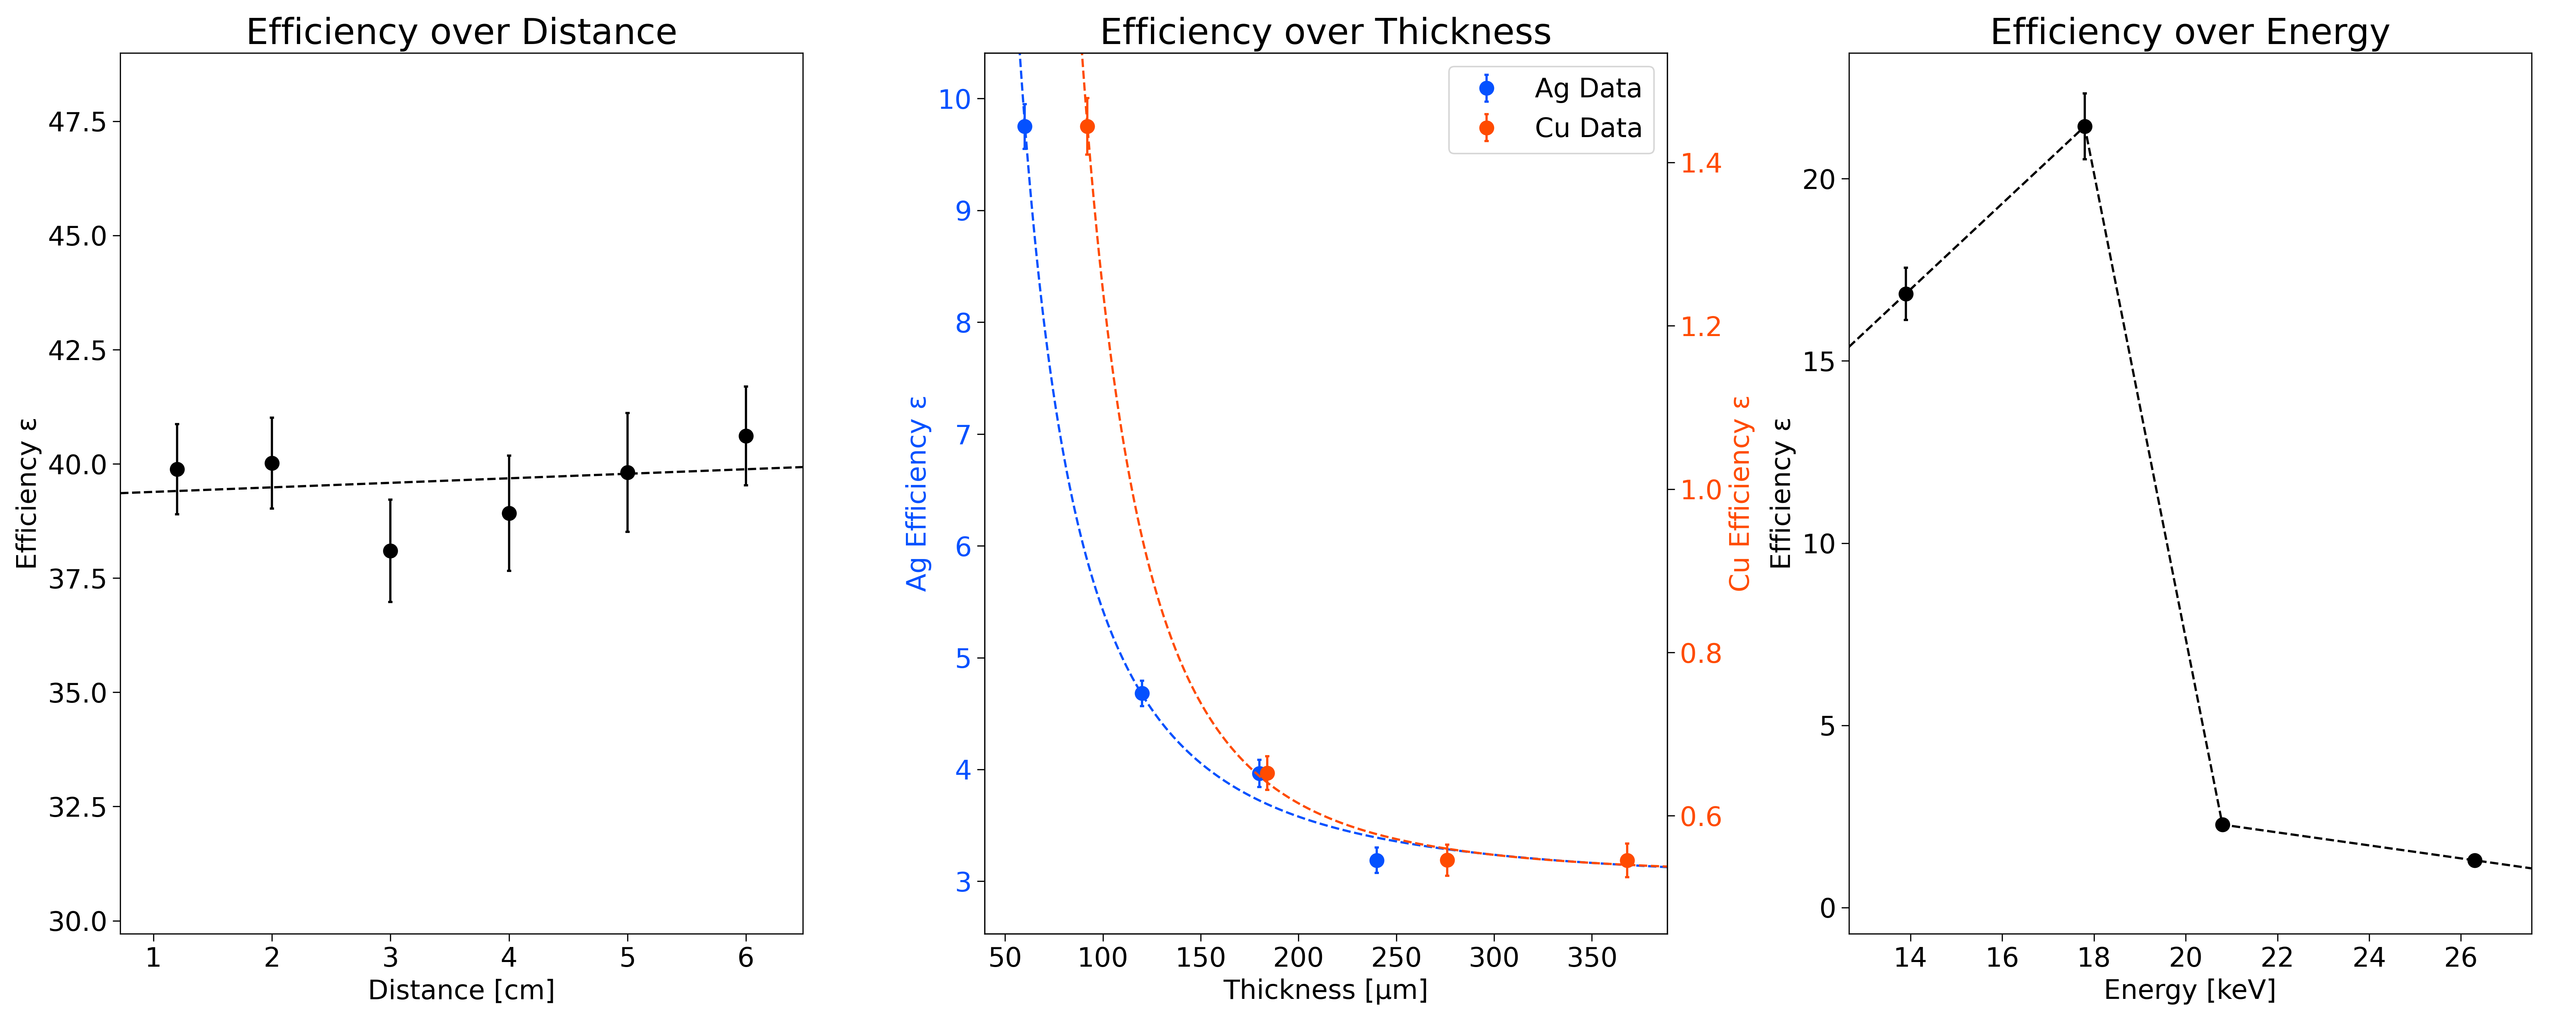
\includegraphics[width=\textwidth]{../Plots/efficiency.png}
   \caption{Curve di efficienza in funzione della distanza tra sorgente e detector (a sinistra), dello spessore di un
            assorbitore (in centro) e in funzione dell'energia dei fotoni (a destra)}
    \label{i:efficiency}
    % \vspace{-10pt}
\end{figure*}

Per costruire la curva di efficienza al variare della distanza tra sorgente e rivelatore, vengono sfruttate le
acquisizioni riportate in \autoref{s:distanza}. In particolare, per ogni spettro raccolto viene calcolata l'efficienza
del picco degli X relativa al picco a $60\,\si{\kilo\electronvolt}$ come in \autoref{e:efficienza}. \\
Per costruire poi la curva di efficienza al variare dello spessore dell'assorbitore tra sorgente e rivelatore si
utilizzano le acquisizioni riportate in \autoref{s:attenuazione}. Si procede quindi in modo analogo alla costruzione
della curva al variare della distanza. \\
Infine, si vuole costruire la curva di efficienza in funzione dell'energia dei fotoni rivelati sfruttando  i risultati
ottenuti mediante il fit multi-picco in \autoref{i:multifit}. A causa dello scarso potere risolvente del rivelatore,
tuttavia, non è possibile isolare dall'istogramma i singoli contributi che compongono il picco degli X, e ci si trova
quindi costretti ad utilizzare le informazioni restituite dal fit. In questo caso, si continua a scegliere il picco a
$60\,\si{\kilo\electronvolt}$ come riferimento in quanto risulta essere l'unico picco ben risolto, dal quale possiamo
trarre informazioni più precise rispetto ai contributi non risolti. Per costruire la curva di efficienza, quindi, viene
calcolato il rapporto di efficienza relativa riportato in \autoref{e:efficienza} per ciascun contributo di raggi X che
compone il picco, sfruttando però i parametri del fit multi-picco, riportati in \autoref{i:multifit}. \\
Le tre curve di efficienza sono riportate in \autoref{i:efficiency}: a sinistra si può osservare l'efficienza relativa
al variare della posizione del detector, in centro si trovano le due curve in funzione dello spessore dell'assorbitore
mentre a destra è raffigurata l'Efficienza relativa in funzione dell'energia dei fotoni emessi. Osservando inizialmente
il primo grafico a sinistra, si può notare come l'efficienza segua un andamento piuttosto costante. Il valore medio è
piuttosto in accordo con il risultato in \autoref{e:efficienza} (la lieve discrepanza può essere legata ad una
statistica meno elevata nell'acquisizione degli spettri al variare della distanza) e, inoltre, la fluttuazione
statistica è in ottimo accordo con le incertezze dell'efficienza. Dalla costanza del rapporto di efficienza relativa
$\text{N}_{\text{X}}/\text{N}_{\gamma}$, si può quindi dedurre che la distanza tra sorgente e detector influenza in
ugual modo la rivelazione degli X e dei $\gamma$. Osservando invece il grafico centrale, è evidente come l'efficienza
relativa segue un forte andamento decrescente: in particolare, la differenza di andamento tra i due materiali è
influenzata dal diverso coefficiente di assorbimento. Il grafico prova chiaramente, quindi, che i raggi $\gamma$ sono
molto più penetranti rispetto agli X: dallo spettro in \autoref{i:spettro_abs}, infatti, si nota che in presenza di un
assorbitore di rame spesso $368\,\si{\micro\metre}$ il rapporto di rivelazione tra raggi X e raggi $\gamma$ è molto
diverso rispetto a quanto ritrovato in \autoref{i:spettro} senza assorbitore. Il picco corrispondente agli X, infatti,
risulta ora essere addirittura più basso del picco a $60\,\si{\kilo\electronvolt}$, evidenziando come i fotoni meno
energetici vengano bloccati più facilmente rispetto a quelli più energetici. Osservando infine il grafico a destra in
\autoref{i:efficiency}, ovvero la curva di efficienza in funzione dell'energia, è complicato trarre conclusioni data la
scarsa quantità di informazione a disposizione: i contributi gaussiani presi in considerazione non sono in numero
sufficiente da far emergere un trend evidente. Inoltre, il range di energie in gioco è piuttosto ristretto, ed il basso
potere risolvente dell'apparato costringe la curva ad essere fortemente dipendente dai parametri del fit multi-picco
(\autoref{i:multifit}), che descrive però in modo solo approssimativo il profilo dello spettro. Infine, è opportuno
evidenziare che per poter ricavare delle informazioni soddisfacenti sull'efficienza del detector in funzione
dell'energia, sarebbe necessario conoscere almeno l'attività della sorgente. 

\pagebreak 

\begin{figure}
    \centering
    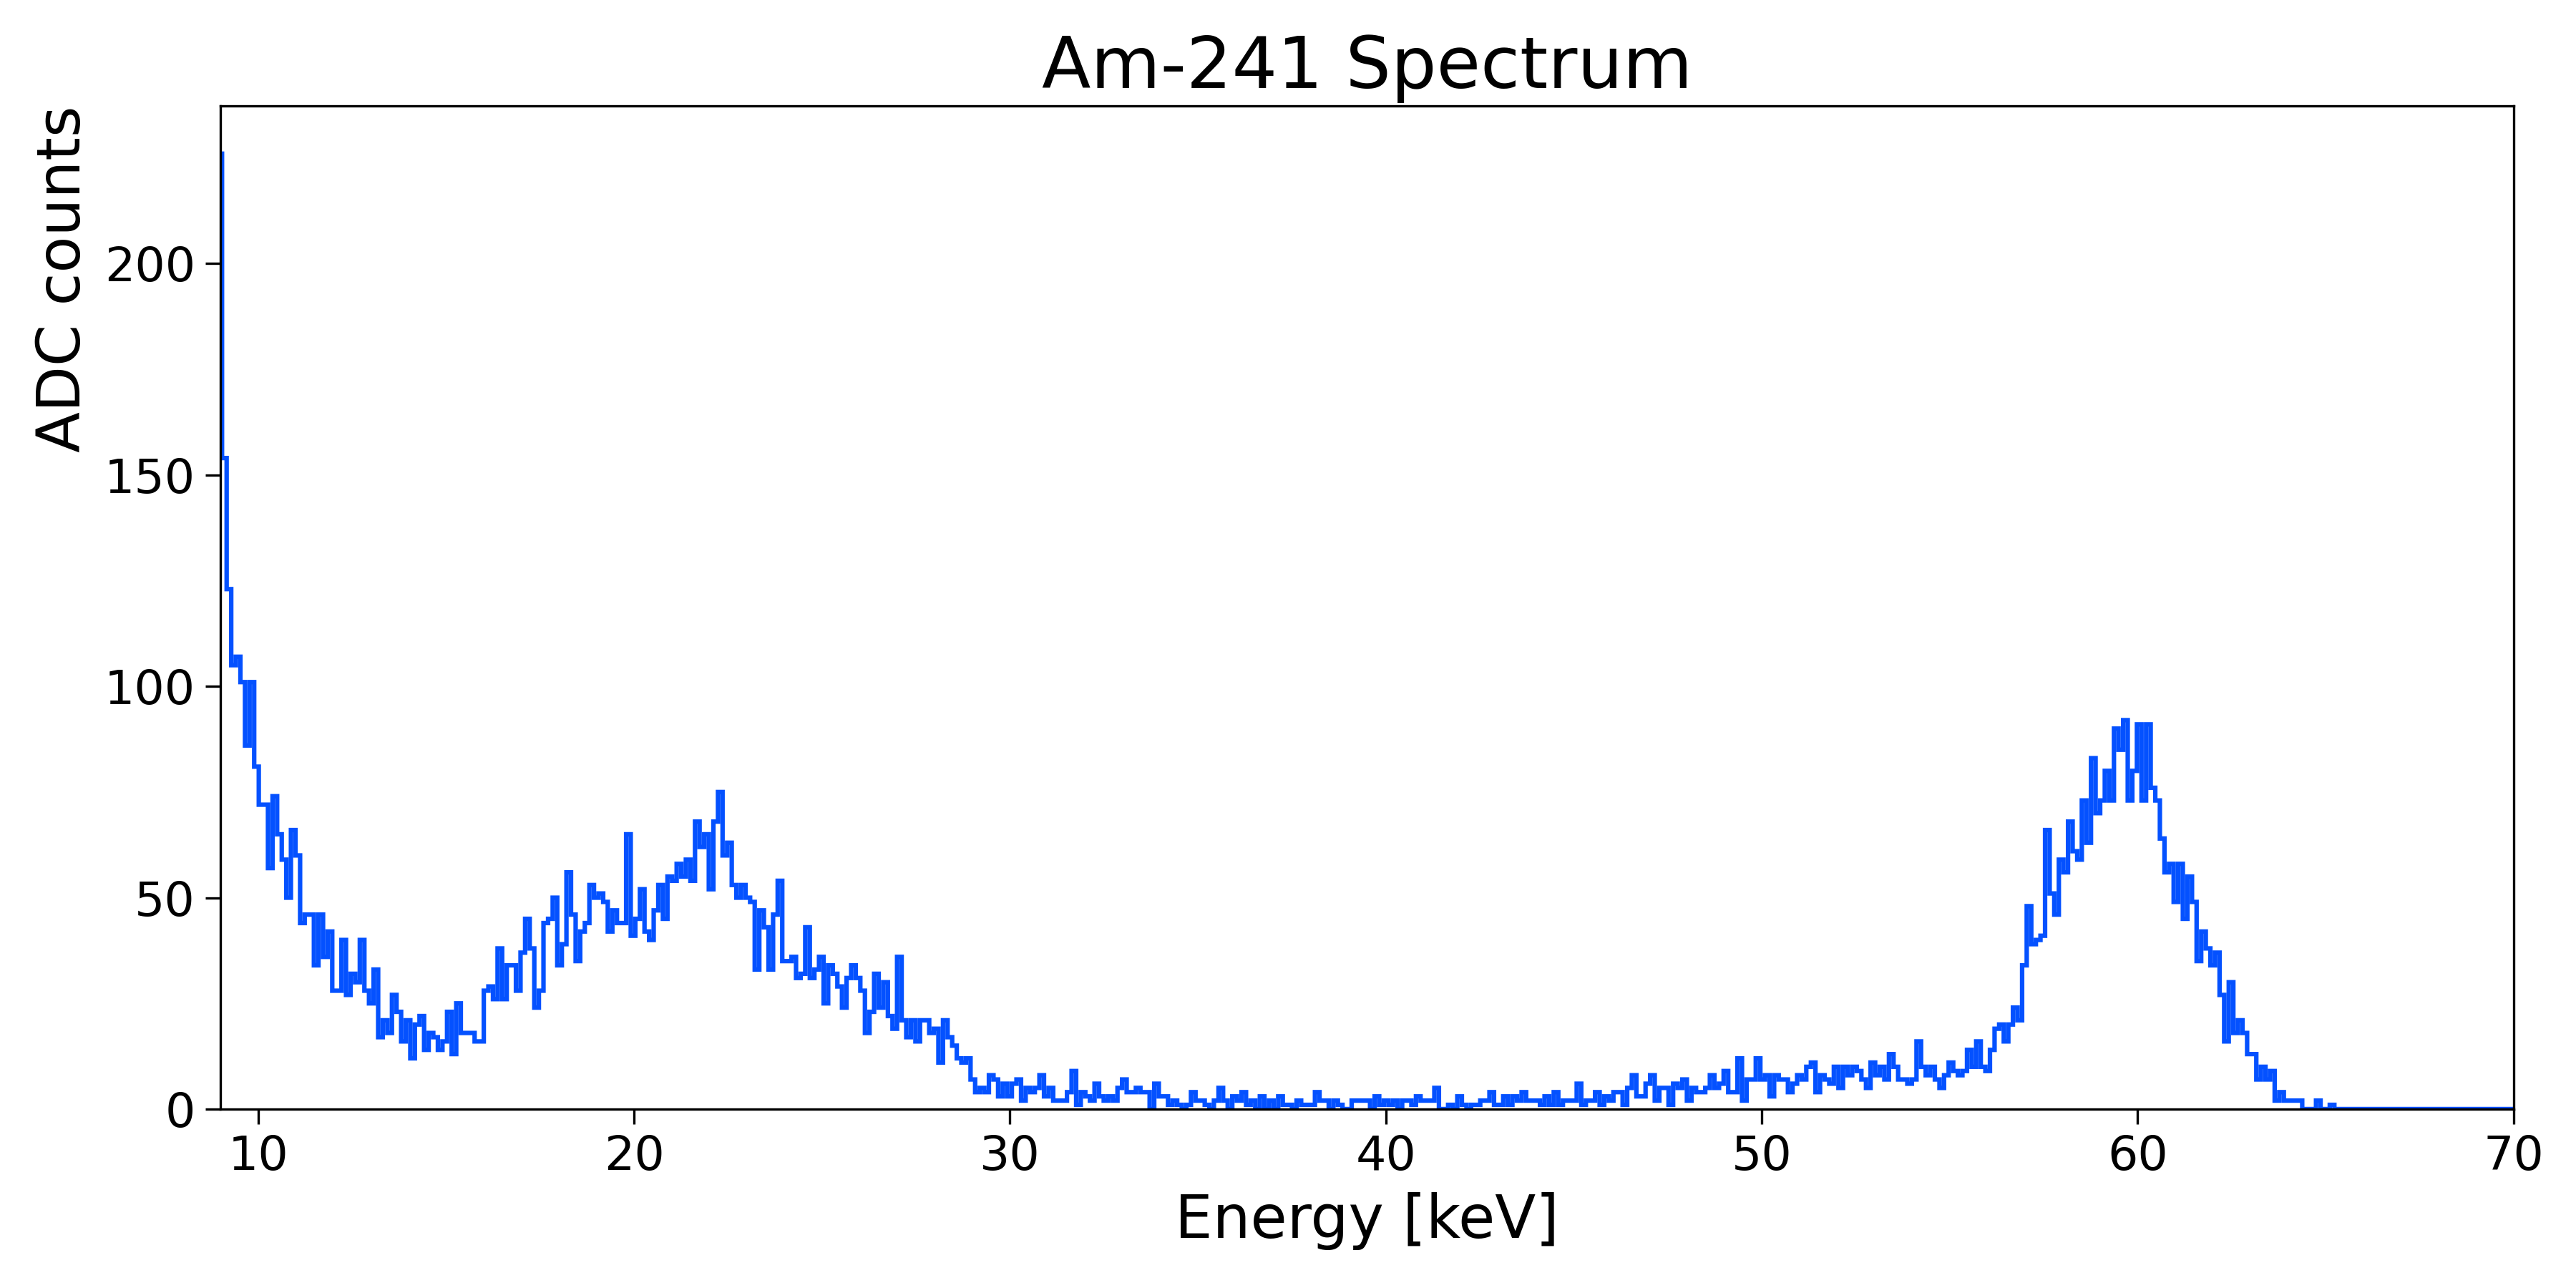
\includegraphics[width=\linewidth]{../Plots/am_spectrum_absorber.png}
    \caption{Spettro dell'Am-241 con assorbitore di rame di spessore $368\,\si{\micro\metre}$}
    \label{i:spettro_abs}
    \vspace{-10pt}
\end{figure}

\null
\vfill

\end{document}
